% !TEX root = /home/computer/ucsc/master-2/quarter-1/machine-learning/master.tex
\assignment{1}{Mon 11 Oct 2021 20:32}{Assignment 1}
\subsectionfont{\fontsize{10}{10}\selectfont}

\section{Problem 1}%
For an adult learning a foreign language, we could consider
two different models for learning to speak and for learning to understand.
Considering the adult already knows a language, learning to speak another
language might require first realizing what the speaker wants to say in their
native language and then translating it to another. Alternatively, learning to
understand a foreign language, would require taking the foreign language and
then translating it into the native language. The following is an example of
a learner learning to speak spanish.

\begin{itemize}
  \item Speaking - How do I say, "I need to go to the bathroom" $\implies$ "Necessito ir al bano"
\end{itemize}

For learning to speak, the features or domain objects would be a list of sentences,
nouns, verbs, idioms, etc in the native language with labels containing the
translated features.

For learning to understand, the features and labels would be reversed. Example
below.

\begin{itemize}
  \item Understanding - "Necissito ir al bano" $\implies$ "I need to go to the bathroom"
\end{itemize}

In either case, reinforcement learning would likely be used, and some kind of
algorithm that provides feedback on how accurately translations are made. 

\section{Problem 2}%
\begin{itemize}
  \item[ \textbf{a)} ] \textbf{What is the task?} 
    \par The task is to predict volatility in financial markets in a $10$ 
    minute window.
    \href{https://www.kaggle.com/c/optiver-realized-volatility-prediction/overview/description}{kaggle
    link} 
  \item[ \textbf{b)} ] \textbf{What is the data used to learn a model?} 
    \par The data used is financial order books listing bids and asking price
    of a stock.
  \item[ \textbf{c)} ] \textbf{What is the primary performance measure?} 
    \par Volatility is measured using the $L_2$ norm of log returns of stock
    price. The log return between times $t_1$ and $t_2$ of price of stock $S$

    \[
      r_{t_1,t_2} = \log \left( \frac{S_{t_2}}{S_{t_1}} \right)
    .\] 

    So price volatility is
    \[
      \sigma = \sqrt{ \sum_{t} r_{t-1,t}^{2} }
    .\] 

    Thus, performance would be measured in how accurately the model predicts
    the actual volatility of a stock.
  \item[ \textbf{d)} ] \textbf{What prior assumptions are reasonable to make?} 
    \par In this problem no prior assumptions are reasonable.
  \item[ \textbf{e)} ] \textbf{What kind of learning will be done.} 
    \par supervised learning.
  \item[ \textbf{f)} ] \textbf{} \textbf{Briefly describe the data made
    available} 
    The data contains bid prices and asking prices for a number of
    stocks at various times.
\end{itemize}

\section{Problem 3}%

\begin{enumerate}
  \item[ \textbf{a)}] \textbf{What kind of machine learning problem is this?}
    \par This is a supervised learning model
  \item[\textbf{b)}] \textbf{Is it a predictive task or a descriptive task?}
    \par This is a predictive task.
  \item[\textbf{c)}] \textbf{Are you likely to use a geometric model, a probabilistic
    model, or a logical model?}
    \par Probabilistic model. How likely a person is to have a certain blood
    pressure
  \item[\textbf{d)}] \textbf{Will your model be a grouping model or a grading model?}
    \par Either could work, but I would like to assign a "grade" to a person.
  \item[\textbf{e)}] \textbf{What is the label space for this problem?}
    \par The label space is two numbers for systolic and diastolic blood
    pressure.
  \item[\textbf{f)}] \textbf{What is the output space for this problem?}
    \par The output space is the same as the label space.
\end{enumerate}

\section{Problem 4}
\begin{itemize}
  \item[ \textbf{a)} ] \textbf{L1 norm} 
    \[
    \boxed{6.3}
    .\] 
  \item[ \textbf{b)} ]\textbf{L2 norm}
    \[
    \boxed{3.62629}
    .\] 
  \item[ \textbf{c)} ]\textbf{L10 norm}
    \[
    \boxed{3.20016}
    .\] 
  \item[ \textbf{d)} ]\textbf{L100 norm}
    \[
    \boxed{3.2}
    .\] 
  \item[ \textbf{e)} ] \textbf{If a constant vector is added to both $x1$ and
    $x2$ which norms will change?} 
    \par Neither will change since,
    \[
      (x_1+v)-(x_2+v) = x_1-x_2
    .\] 
  \item[ \textbf{f)} ] \textbf{If multiplied by a constant $k$} 
    \par All of them will change by properties of norms unless $k=\pm1$
    \[
      \|kx_1-kx_2\|_{p} = |k|\|x_1-x_2\|_{p}
    .\] 
\end{itemize}

\section{Problem 5}%

Joint probability distribution for class machine learning. Total class size is
$410$

\[
\begin{tabular}{c | c | c | c | c}
  grade & effort = small & medium & large & margin \\
  \hline \\
  A & $ \textcolor{WildStrawberry}{0}
  $ & $ \textcolor{WildStrawberry}{\frac{25}{410}
  } $ & $ \textcolor{WildStrawberry}{\frac{75}{410}} $ & $ \textcolor{BlueGreen}{\frac{100}{410}} $\\ \\
  \hline \\
  B & $ \textcolor{WildStrawberry}{\frac{5}{410}}$ & $\textcolor{WildStrawberry}{\frac{50}{410}} $ & $\textcolor{WildStrawberry}{\frac{50}{410}} $ & $ \textcolor{BlueGreen}{\frac{105}{410}} $\\ \\
  \hline \\
  C & $ \textcolor{WildStrawberry}{\frac{25}{410}}
  $ & $ \textcolor{WildStrawberry}{\frac{50}{410}}
  $ & $ \textcolor{WildStrawberry}{\frac{5}{410}} $ & $ \textcolor{BlueGreen}{\frac{80}{410}} $\\\\
  \hline \\
  D & $ \textcolor{WildStrawberry}{\frac{50}{410}}
  $ & $ \textcolor{WildStrawberry}{\frac{25}{410}}
  $ & $ \textcolor{WildStrawberry}{0} $ & $ \textcolor{BlueGreen}{\frac{75}{410}} $\\\\
  \hline \\
  F & $ \textcolor{WildStrawberry}{\frac{50}{410}}
  $ & $ \textcolor{WildStrawberry}{0} $ & $ \textcolor{WildStrawberry}{0}
  $ & $ \textcolor{BlueGreen}{\frac{50}{410}} $ \\\\ 
  \hline \\
  margin & $ \textcolor{Orchid}{\frac{130}{410}}
  $ & $ \textcolor{Orchid}{\frac{150}{410}} $ & $ \textcolor{Orchid}{\frac{130}{410}} $ & $100\%$
\end{tabular}
.\] 

The joint probability distribution for class surfing with total class size $500$

\[
\begin{tabular}{c | c | c | c | c}
  grade & effort = small & medium & large & margin \\
  \hline \\
 A & $ \textcolor{WildStrawberry}{\frac{50}{500}}$
   & $ \textcolor{WildStrawberry}{ \frac{125}{500}}
 $ & $ \textcolor{WildStrawberry}{\frac{125}{500}}
 $ & $ \textcolor{BlueGreen}{\frac{300}{500}} $ \\\\
 \hline \\
 B & $ \textcolor{WildStrawberry}{\frac{50}{500}}
 $ & $ \textcolor{WildStrawberry}{\frac{50}{500}}
 $ & $\textcolor{WildStrawberry}{\frac{25}{500}}$
   & $ \textcolor{BlueGreen}{\frac{125}{500}} $ \\\\
 \hline \\
 C & $ \textcolor{WildStrawberry}{\frac{50}{500}}
 $ & $ \textcolor{WildStrawberry}{\frac{25}{500}}
 $ & $ \textcolor{WildStrawberry}{0} $ & $\textcolor{BlueGreen}{\frac{75}{500}}
 $\\ \\
 \hline \\
 D & $ \textcolor{WildStrawberry}{0}$ & $ \textcolor{WildStrawberry}{0}$
   & $ \textcolor{WildStrawberry}{0}$ & $ \textcolor{BlueGreen}{0}$ \\ \\
 \hline \\
 F & $ \textcolor{WildStrawberry}{0}$ & $ \textcolor{WildStrawberry}{0}$
   & $ \textcolor{WildStrawberry}{0}$ & $ \textcolor{BlueGreen}{0}$ \\ \\
 \hline \\
 margin & $ \textcolor{Orchid}{\frac{150}{500}}
 $ & $ \textcolor{Orchid}{\frac{200}{500}}
 $ & $ \textcolor{Orchid}{\frac{150}{500}}$ & $100\%$
\end{tabular}
.\] 

\begin{itemize}
  \item[ \textbf{a)} ] \textbf{What is the conditional probability distribution P(grade|class,effort)} 
    \par The conditional probability distribution for each class are the items
    labeled in \textcolor{WildStrawberry}{red} in the tables above.
  \item[ \textbf{b) and c)}] \textbf{What is the marginal probability distribution
    P(grade,effort)} 
    \par The marginal probabilities of grade for each class are the
    \textcolor{BlueGreen}{blue} columns on the right of each table, and for
    effort are the \textcolor{Orchid}{purple} rows on the bottom of each table
  \item[ \textbf{d)} ] \textbf{P(grade=A|class)} 
    \par For class machine learning this is
    $ \textcolor{BlueGreen}{\frac{100}{410}} $ and for class surfing this is
    $ \textcolor{BlueGreen}{\frac{300}{500}} $
\end{itemize}


\section{Problem 6}%

Plotting the feature space

\graphicspath{ {/home/computer/ucsc/master-2/quarter-1/machine-learning/assignment_01/figures/} }
\begin{figure}[H]
    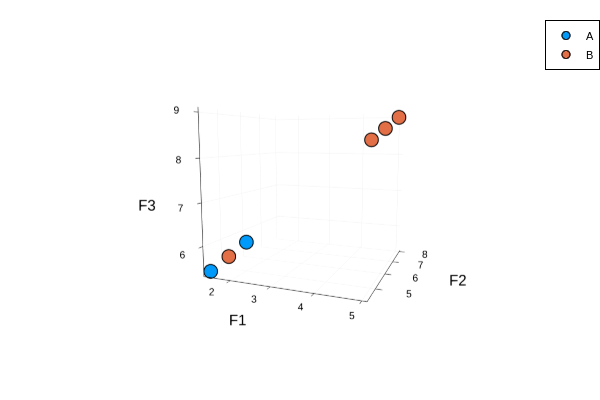
\includegraphics[width=0.8\linewidth]{plot.png}
\end{figure}

\begin{itemize}
  \item[ \textbf{a)} ] \textbf{Intrinsic dimensionality} 
    \par From the plot we can see that the data has intrinsic dimensionality of
    1
  \item[ \textbf{b)} ] \textbf{Geometric discriminating function in two
    dimensional feature space} 
    \par The separating function would be a plane
  \item[ \textbf{c)}] \textbf{Are these  examples linearly separable in the
    intrinsic feature space?} 
    \par We can see visually from the plot that these examples are not linearly
    separable
  \item[ \textbf{d)} ] \textbf{Linearly separable in original feature space?}
    \par Again, from the plot, we can see that these examples are not linearly
    separable.
\end{itemize}

\section{Problem 7}%
From highest to lowest $\{x_{i}\}$ is ranked in the following order where items
colored \textcolor{WildStrawberry}{red} are in the negative class and items
colored in \textcolor{BlueGreen}{blue} are in the positive class
\[
\textcolor{BlueGreen}{x_9}, \textcolor{BlueGreen}{x_{10}},
\textcolor{BlueGreen}{x_{12}}, \textcolor{BlueGreen}{x_{11}},
\textcolor{BlueGreen}{x_{7}}, \textcolor{WildStrawberry}{x_{15}},
\textcolor{BlueGreen}{x_4}, \textcolor{BlueGreen}{x_2},
\textcolor{BlueGreen}{x_3}, \textcolor{WildStrawberry}{x_{22}},
\textcolor{WildStrawberry}{x_{16}}, \textcolor{WildStrawberry}{x_{19}},
\textcolor{WildStrawberry}{x_{25}}, \textcolor{WildStrawberry}{x_{23}},
\textcolor{WildStrawberry}{x_{24}}, \textcolor{BlueGreen}{x_1},
\textcolor{BlueGreen}{x_5}, \textcolor{WildStrawberry}{x_{13}},
\textcolor{BlueGreen}{x_6}, \textcolor{BlueGreen}{x_8},
\textcolor{WildStrawberry}{x_{14}}, \textcolor{WildStrawberry}{x_{21}},
\textcolor{WildStrawberry}{x_{17}}, \textcolor{WildStrawberry}{x_{20}},
\textcolor{WildStrawberry}{x_{18}} 
.\] 
\begin{itemize}
  \item[ \textbf{a)} ] \textbf{How many ranking errors are there?} 
    \par $\underbrace{1}_{\textcolor{BlueGreen}{x_4}}
    + \underbrace{1}_{\textcolor{BlueGreen}{x_2}}
    + \underbrace{1}_{\textcolor{BlueGreen}{x_3}}
    + \underbrace{7}_{\textcolor{BlueGreen}{x_1}}
    + \underbrace{7}_{\textcolor{BlueGreen}{x_5}}
    + \underbrace{8}_{\textcolor{BlueGreen}{x_6}}
    + \underbrace{8}_{\textcolor{BlueGreen}{x_8}} = \boxed{33}$
  \item[ \textbf{b)} ] Ranking error rate?
    \par $\frac{33}{( \textcolor{BlueGreen}{12} )(
    \textcolor{WildStrawberry}{13} )} = \boxed{0.2115}$
  \item[ \textbf{c)} ] Ranking accuracy?
    \par $1-$ error rate  $= \boxed{0.78846}$
\end{itemize}

\section{Problem 8}%

\begin{itemize}
  \item[ \textbf{a)} ] \textbf{Coverage Plot} 
    \begin{figure}[H]
      \centering
      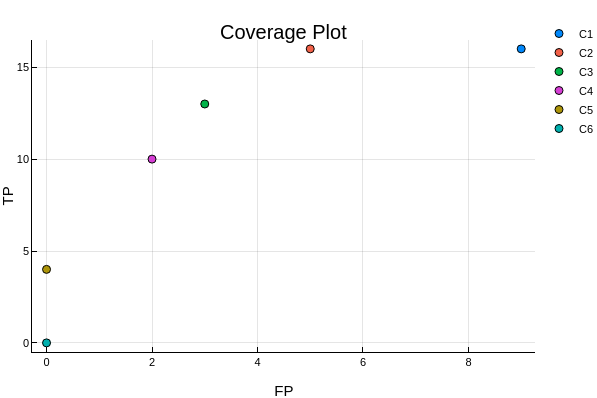
\includegraphics[width=0.8\linewidth]{coverage_plot.png}
    \end{figure}
  \item[ \textbf{b)} ]  \textbf{ROC Plot} 
    \begin{figure}[H]
      \centering
      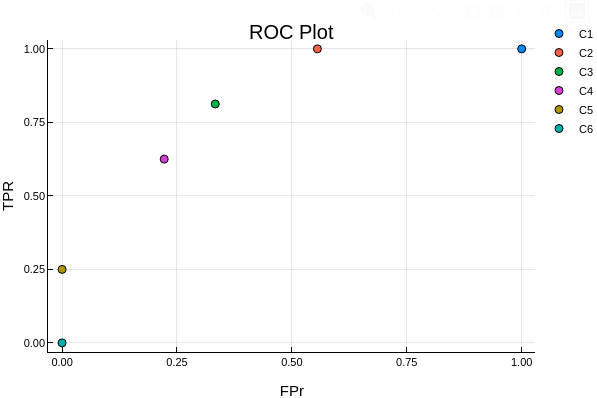
\includegraphics[width=0.8\linewidth]{ROC_plot.png}
    \end{figure}
  \item[ \textbf{c)} ] \textbf{Which classifiers have the highest and lowest
    accuracy?} 
    \par Highest: C2; Lowest: C6
  \item[ \textbf{d)} ] \textbf{Highest and lowest precision?} 
    \par Highest: C5; Lowest: C1
  \item[ \textbf{e)} ]  \textbf{Highest and lowest recall?} 
    \par Highest: C1 and C2; Lowest: C6
  \item[ \textbf{f)}] \textbf{Which classifiers (if any) are complete?} 
    \par classifiers C1 and C2 
  \item[ \textbf{g)}] \textbf{Which classifiers (if any) are consistent?} 
    \par classifiers C5 and C6 
\end{itemize}


